\title{ALPSアプリケーション実行チュートリアル}

\begin{document}

\lstset{language={C++},showspaces=false,rulecolor=\color[cmyk]{0, 0.29,0.84,0}}

\begin{frame}
  \titlepage
\end{frame}

\begin{frame}
   \tableofcontents
\end{frame}

\section{XML入門}

\begin{frame}{ALPSによるシミュレーション --- ワークフロー}
  \begin{center}
    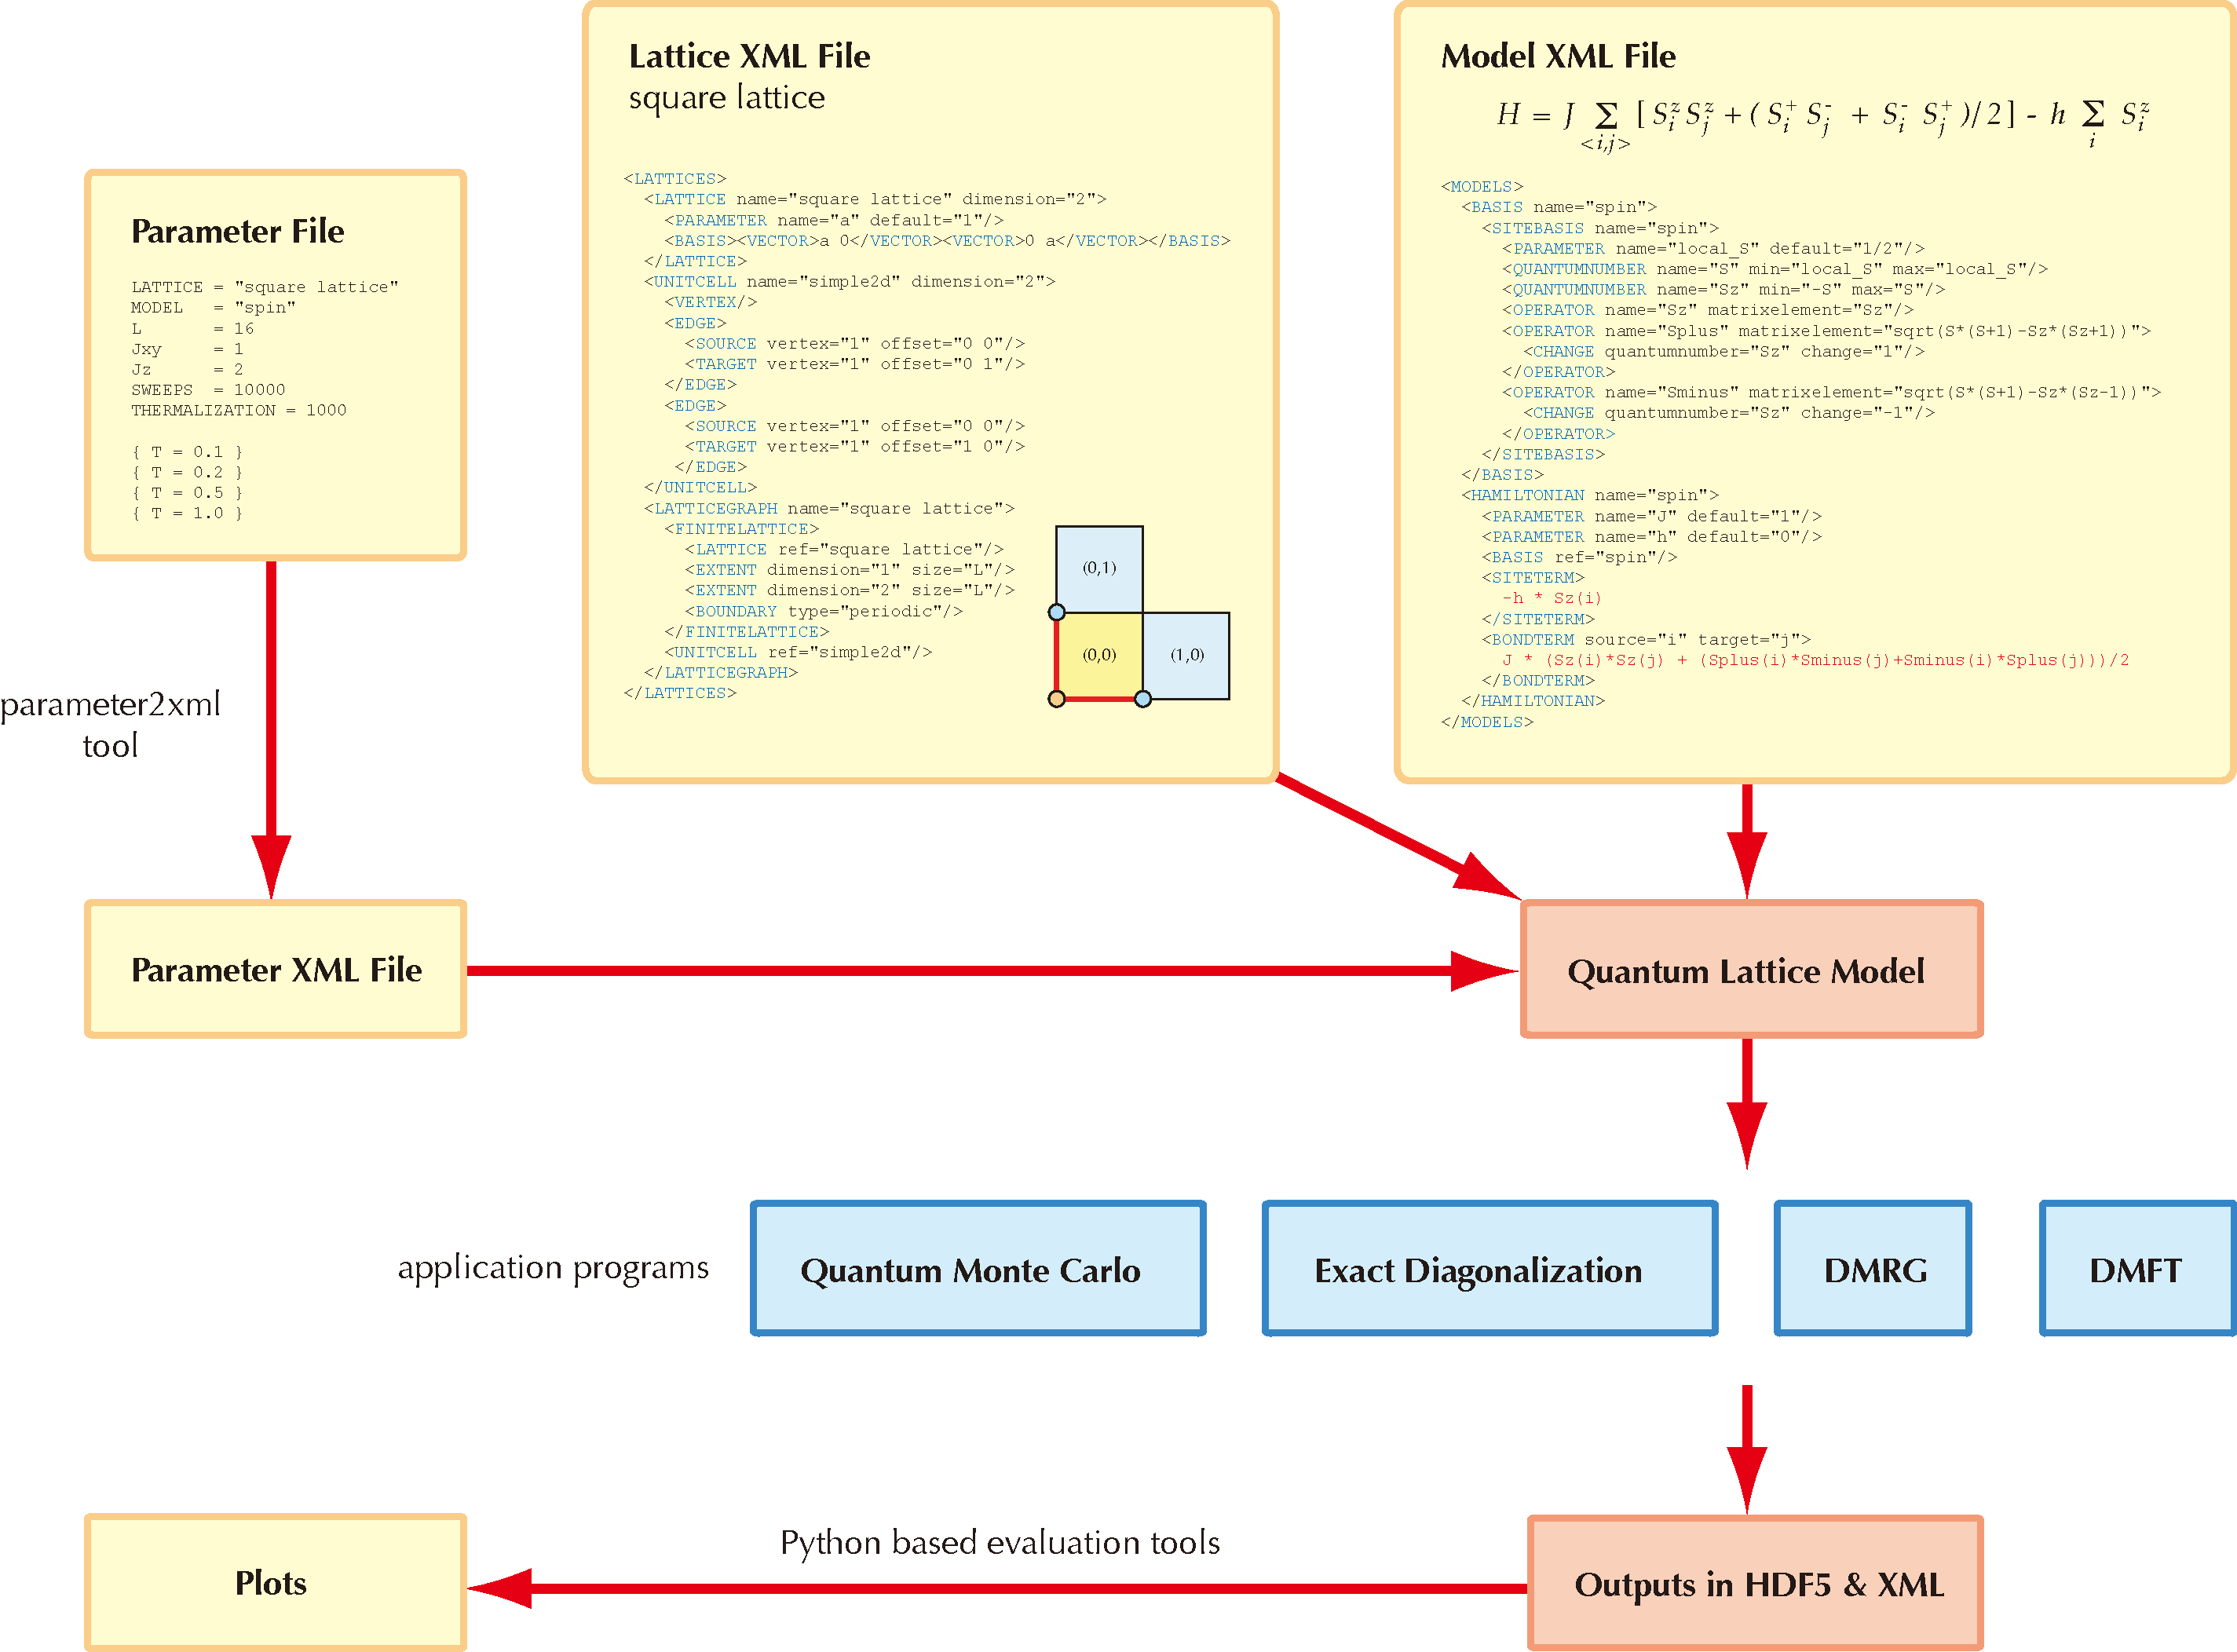
\includegraphics[height=0.8\textheight]{workflow.pdf}
  \end{center}
\end{frame}

\begin{frame}{XMLの基礎}
  \begin{itemize}
  \item XML = e{\color{red} X}tensible {\color{red} M}arckup {\color{red} L}anduage
  \item 構造化文書を作成するのに適している
  \item 「タグ」を使って、文章の構造を記述
  \item 大文字と小文字は区別される
  \item XMLの例: HTML (XHTML)
  \begin{center}
    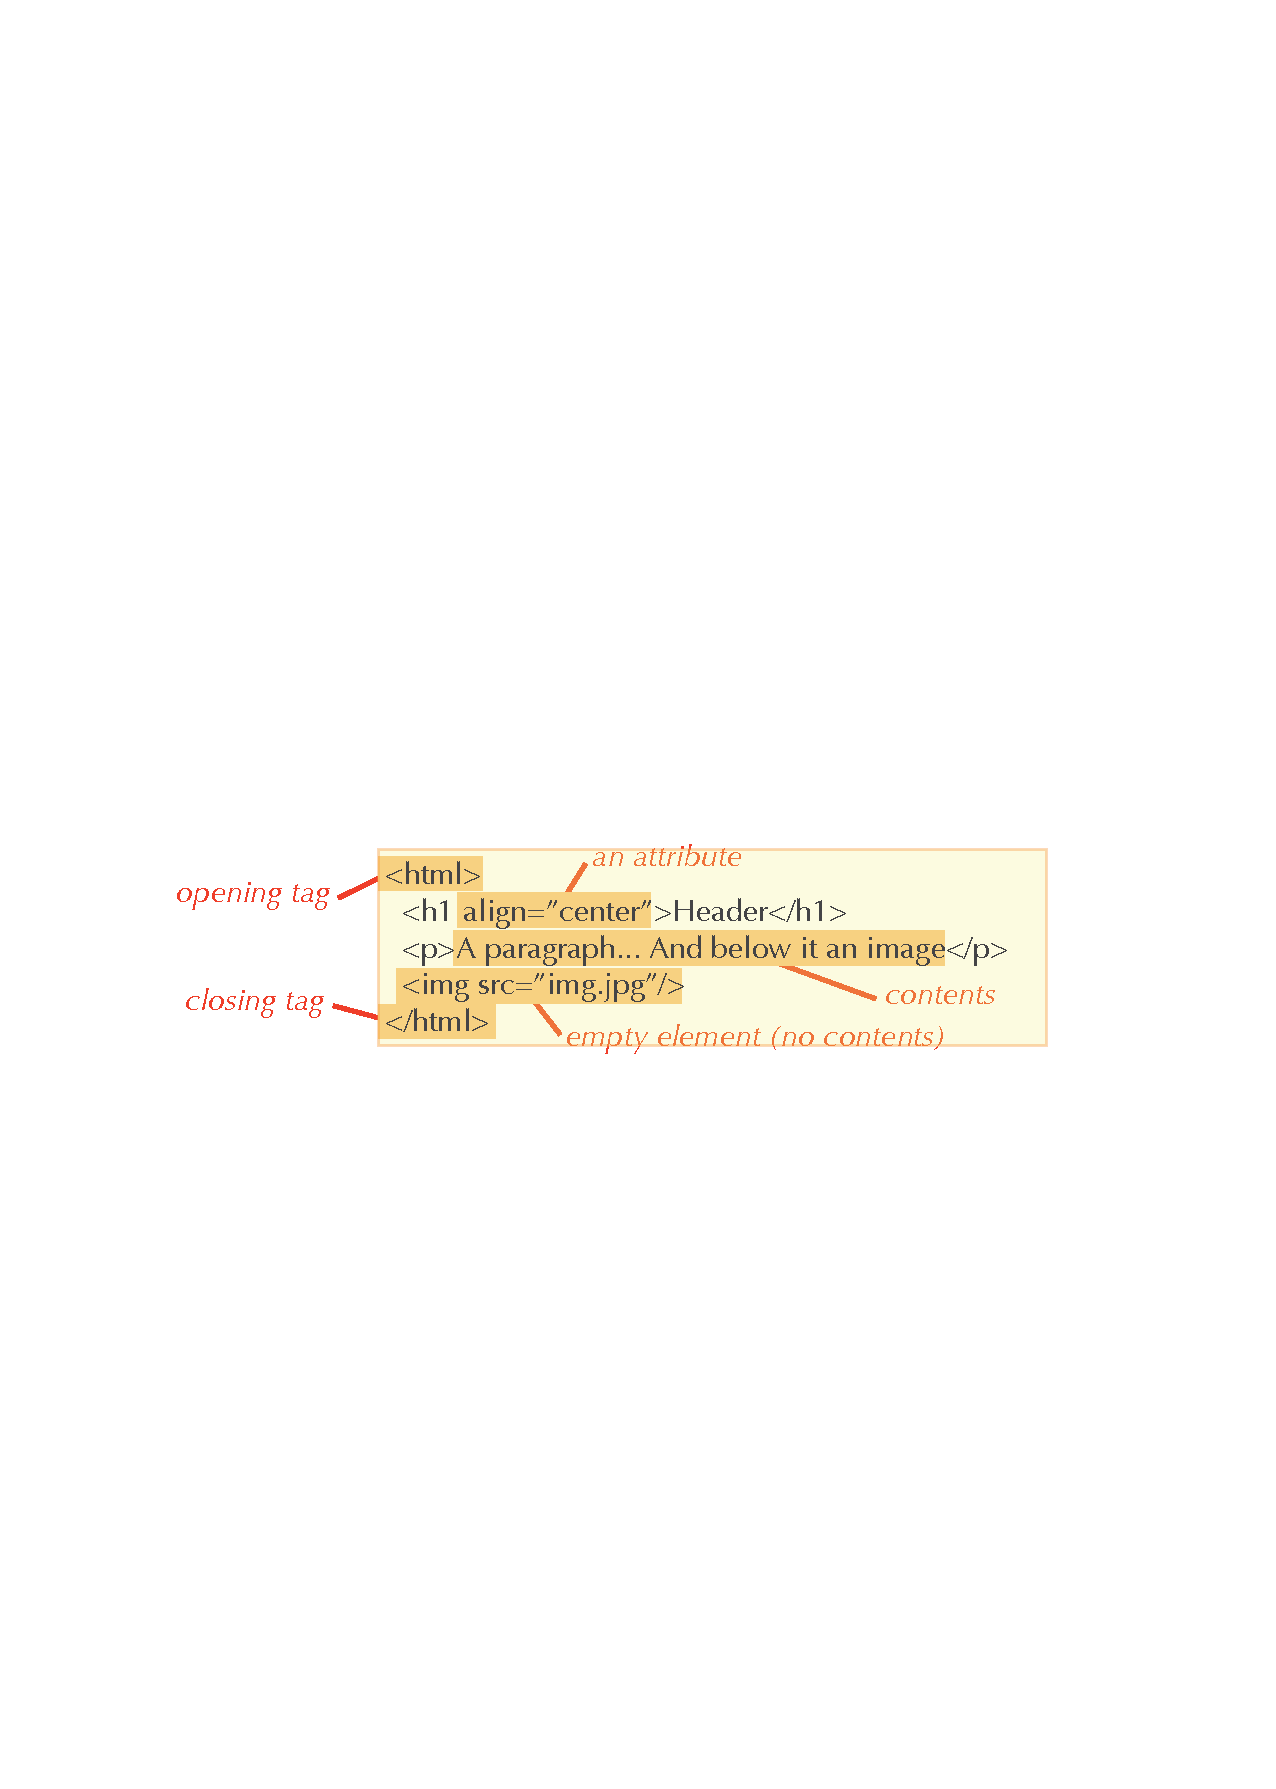
\includegraphics[height=0.3\textheight]{xml1.pdf}
  \end{center}
  \end{itemize}
\end{frame}

\begin{frame}{XMLの文法}
  \begin{itemize}
  \item 「開始タグ」には対応する「終了タグ」が必要
  \item ある要素の「開始タグ」と終了タグは共通の親ノードに含まれなければならない
  \item XMLの「木」表示
  \begin{center}
    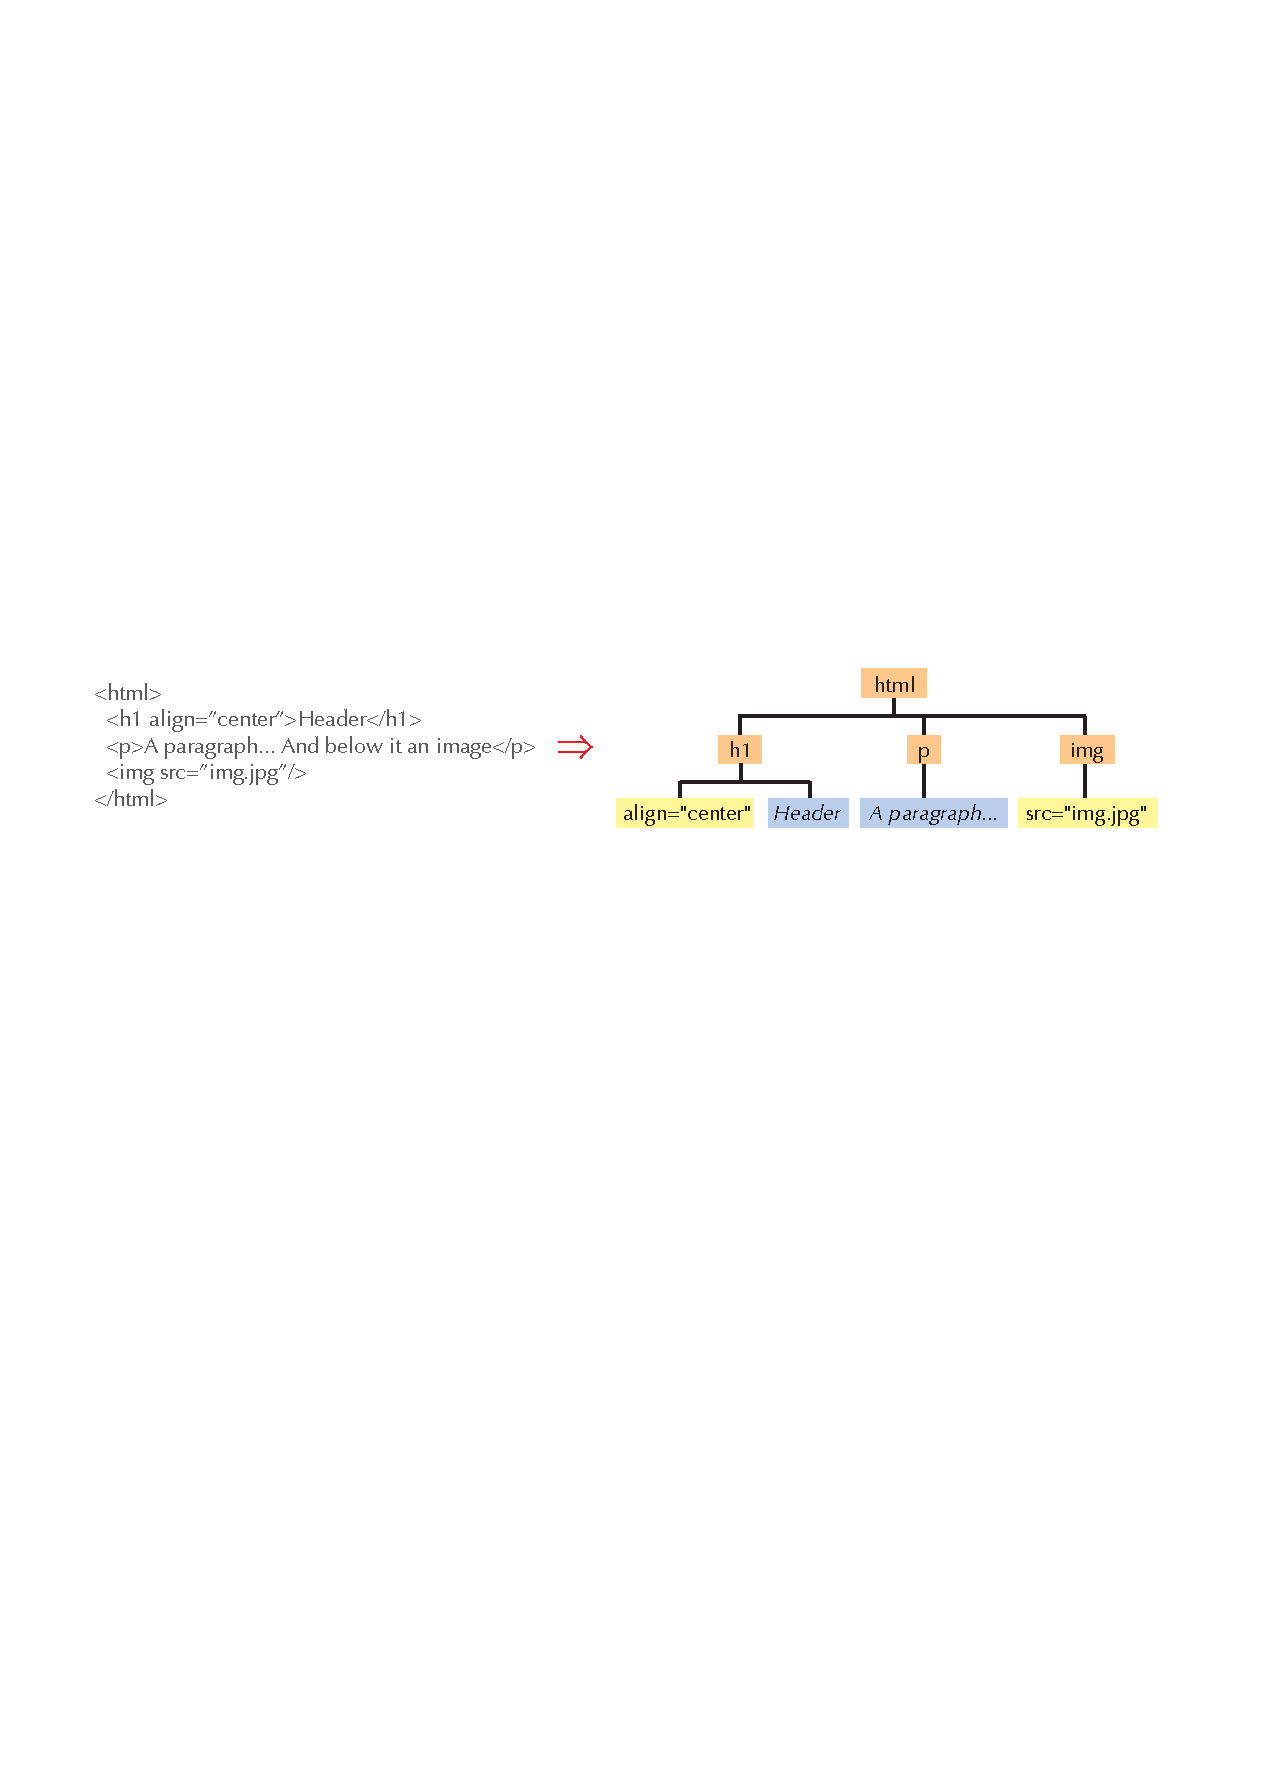
\includegraphics[width=\textwidth]{xml2.pdf}
  \end{center}
  \item XMLでは、ユーザが独自のタグ(要素の名前)を定義することが可能 \\
    (参考: Document Type Definition (DTD), XML Schema)
  \end{itemize}
\end{frame}

\begin{frame}{なぜXMLを使うのか?}
  \begin{center}
    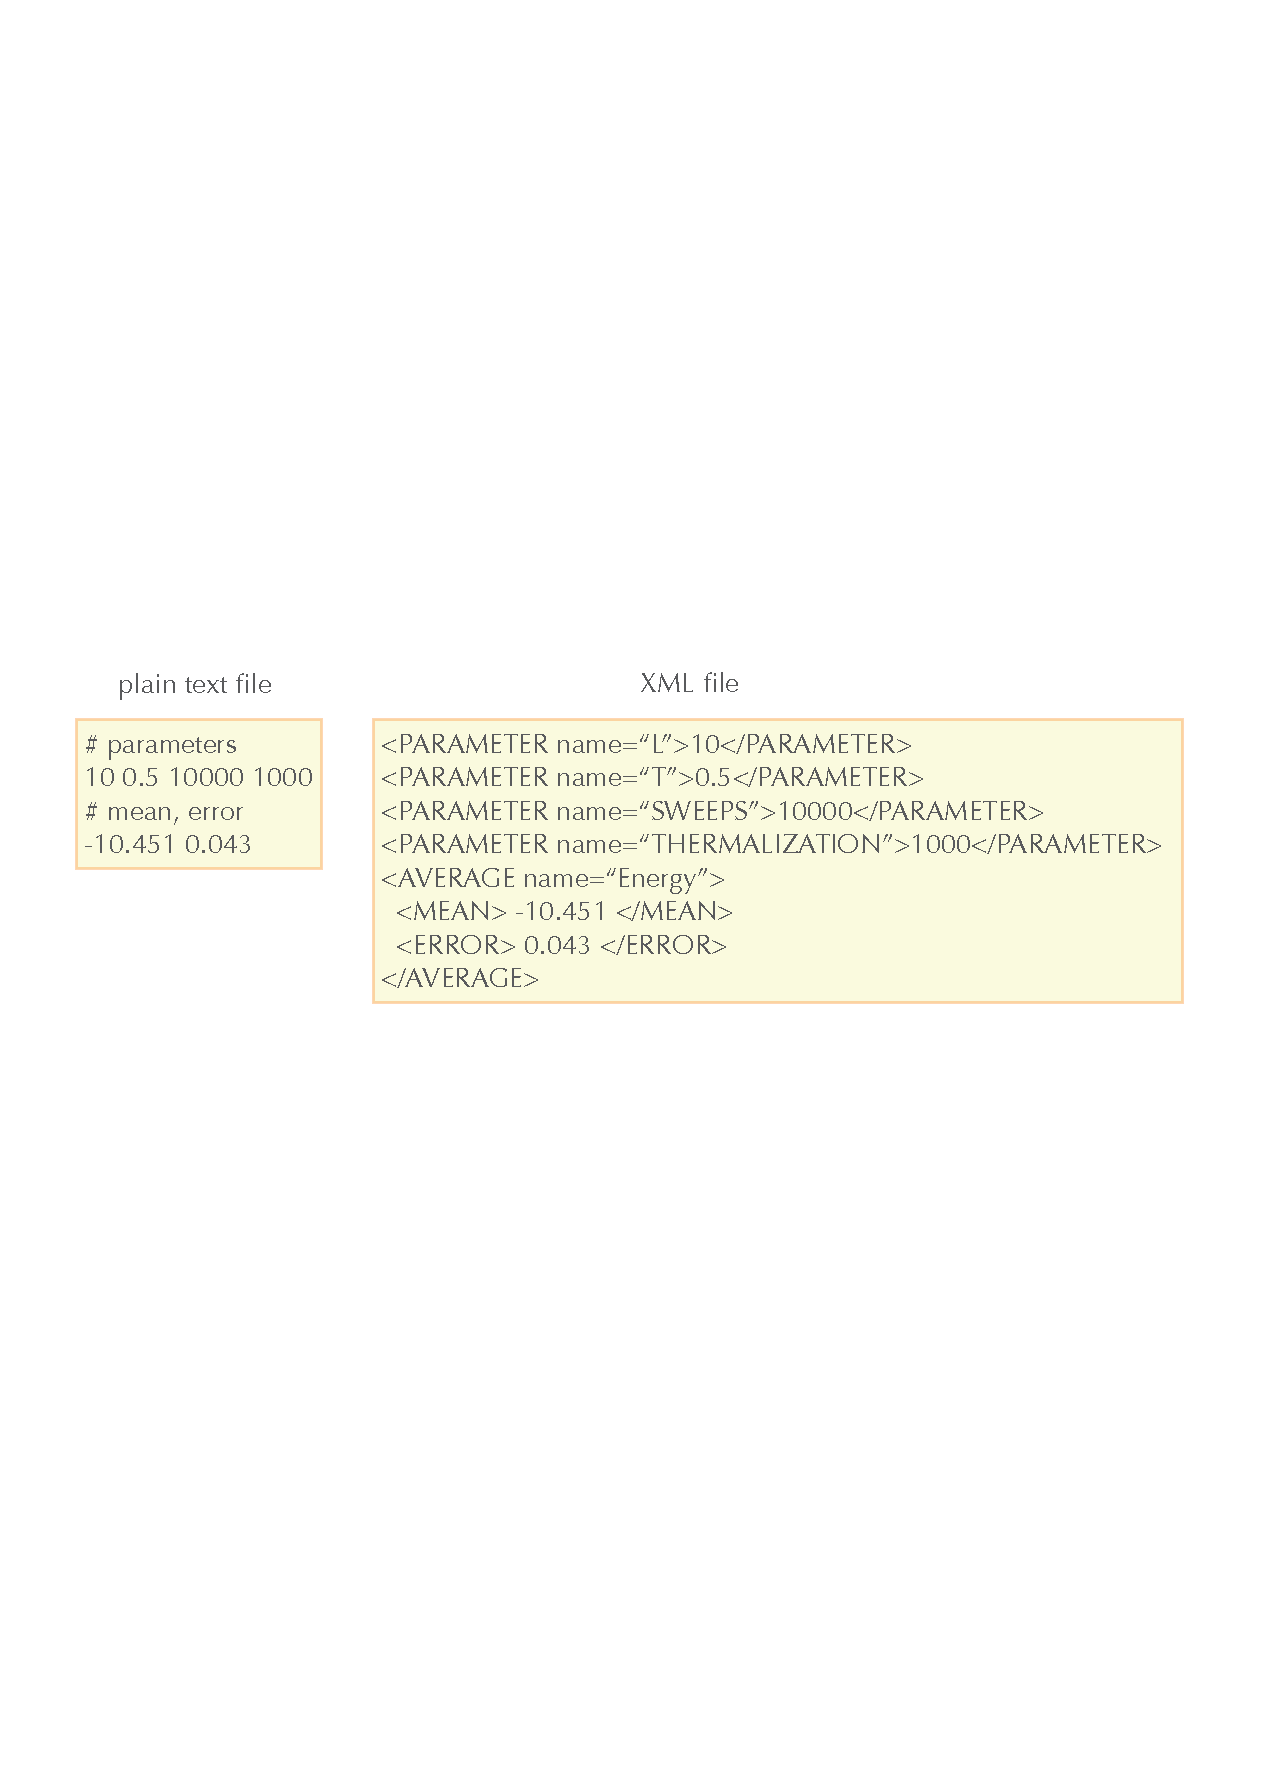
\includegraphics[width=.8\textwidth]{xml3.pdf}
  \end{center}
  \begin{itemize}
  \item 人間にはどちらが読みやすい?
  \item 機械にはどちらがよみやすい?
  \item 数年後に読んで理解できるのはどっち?
  \end{itemize}
\end{frame}

\begin{frame}{データ形式の拡張性}
  \begin{itemize}
  \item 新しいパラメータを追加すると、、、
  \begin{center}
    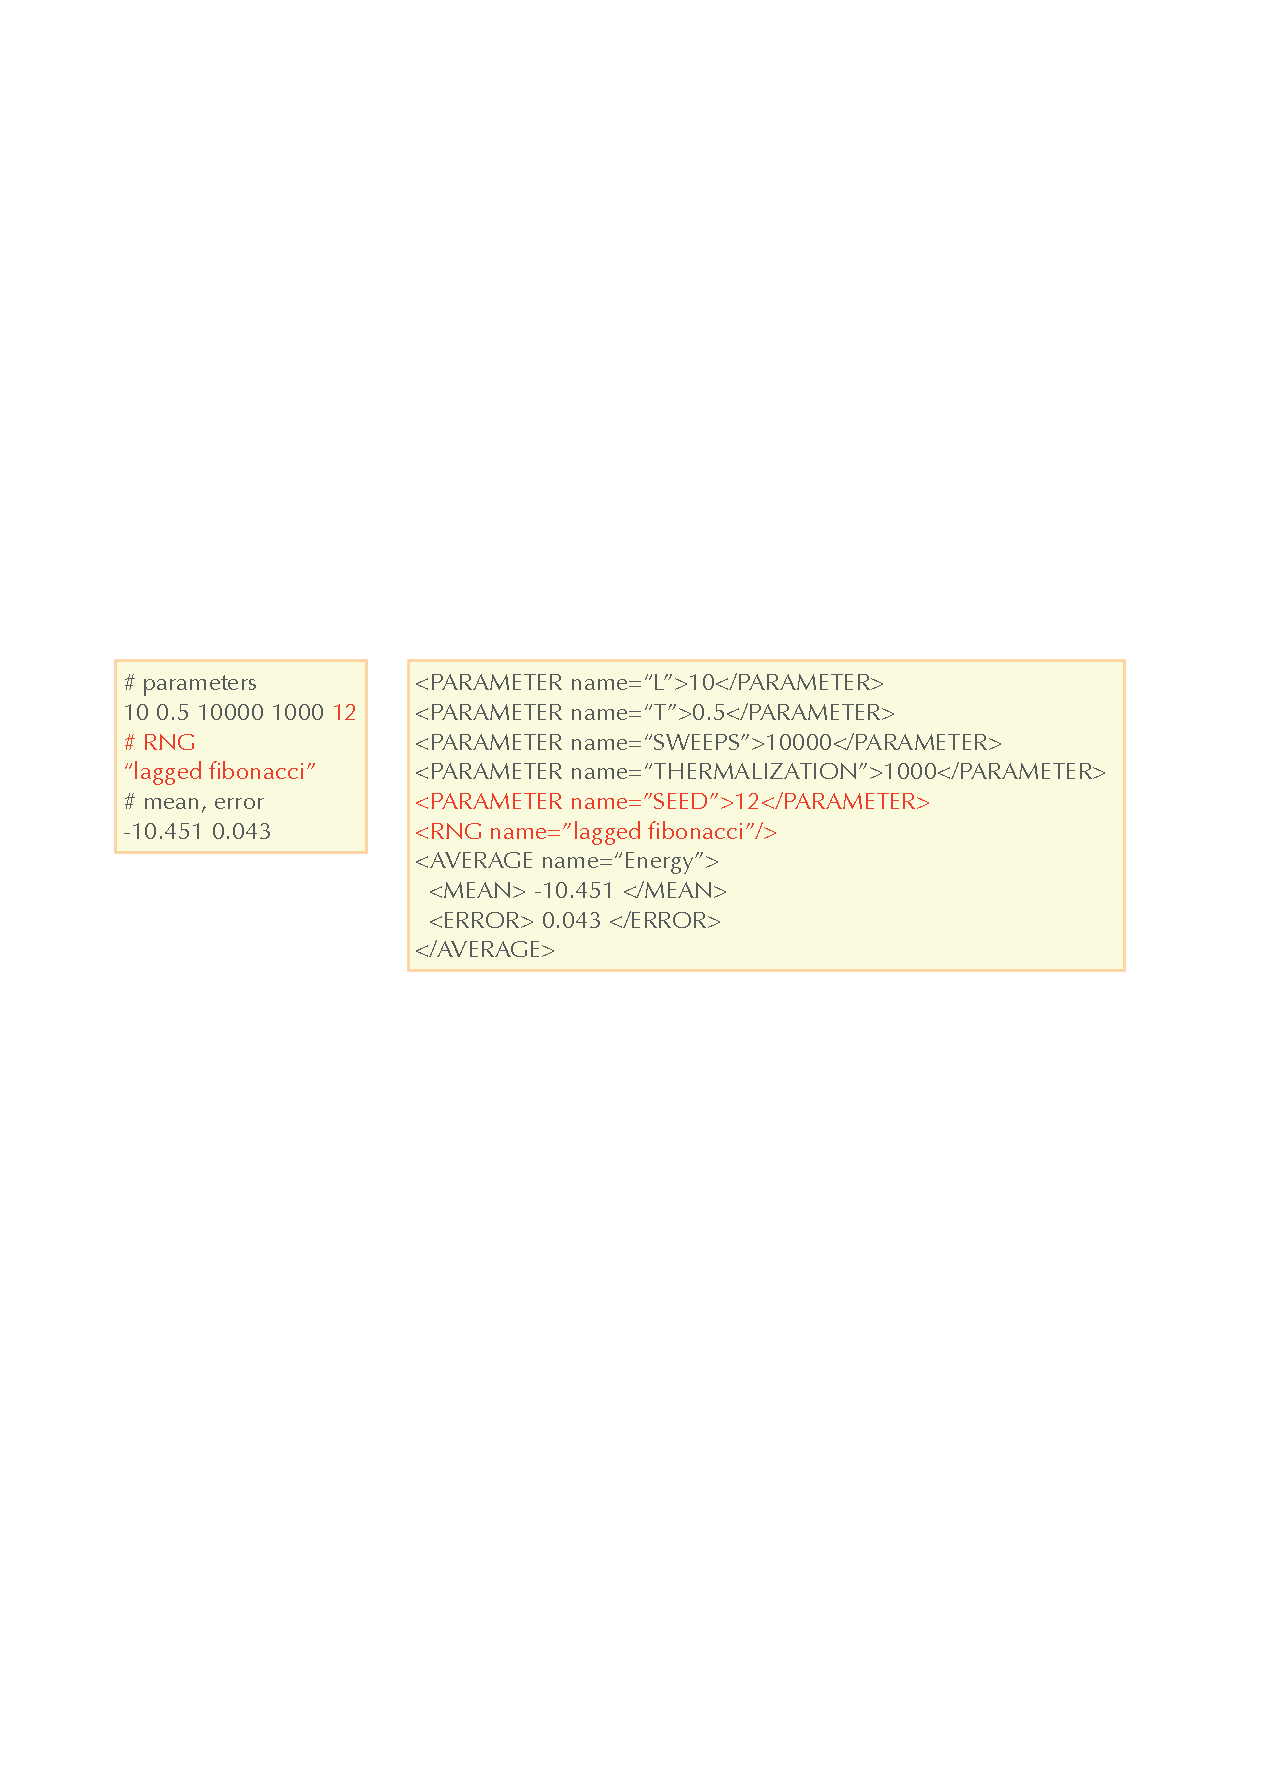
\includegraphics[width=.8\textwidth]{xml4.pdf}
  \end{center}
  \item テキスト形式の場合、これまでのプログラムは動かなくなる
  \item XMLの場合には問題ない (必要のないパラメータは読まれない)
  \end{itemize}
\end{frame}

\section{ALPSシミュレーションの流れ}

\begin{frame}{シミュレーションの入出力}
  \begin{itemize}
  \item 典型的には、一つのシミュレーションは複数のパラメータセットからなる \\ (異なる温度など)
    \begin{itemize}
    \item 「ジョブ(job)」: シミュレーション全体、「タスク」の集合
    \item 「タスク(task)」(または「simulation」):– 一つのパラメータセットに対する計算、「ラン」の集合
    \item 「ラン(run)」(または「clone」): 異なる乱数の種に対する個々の計算
    \end{itemize}
  \item XML入力ファイルと出力ファイル
  \begin{center}
    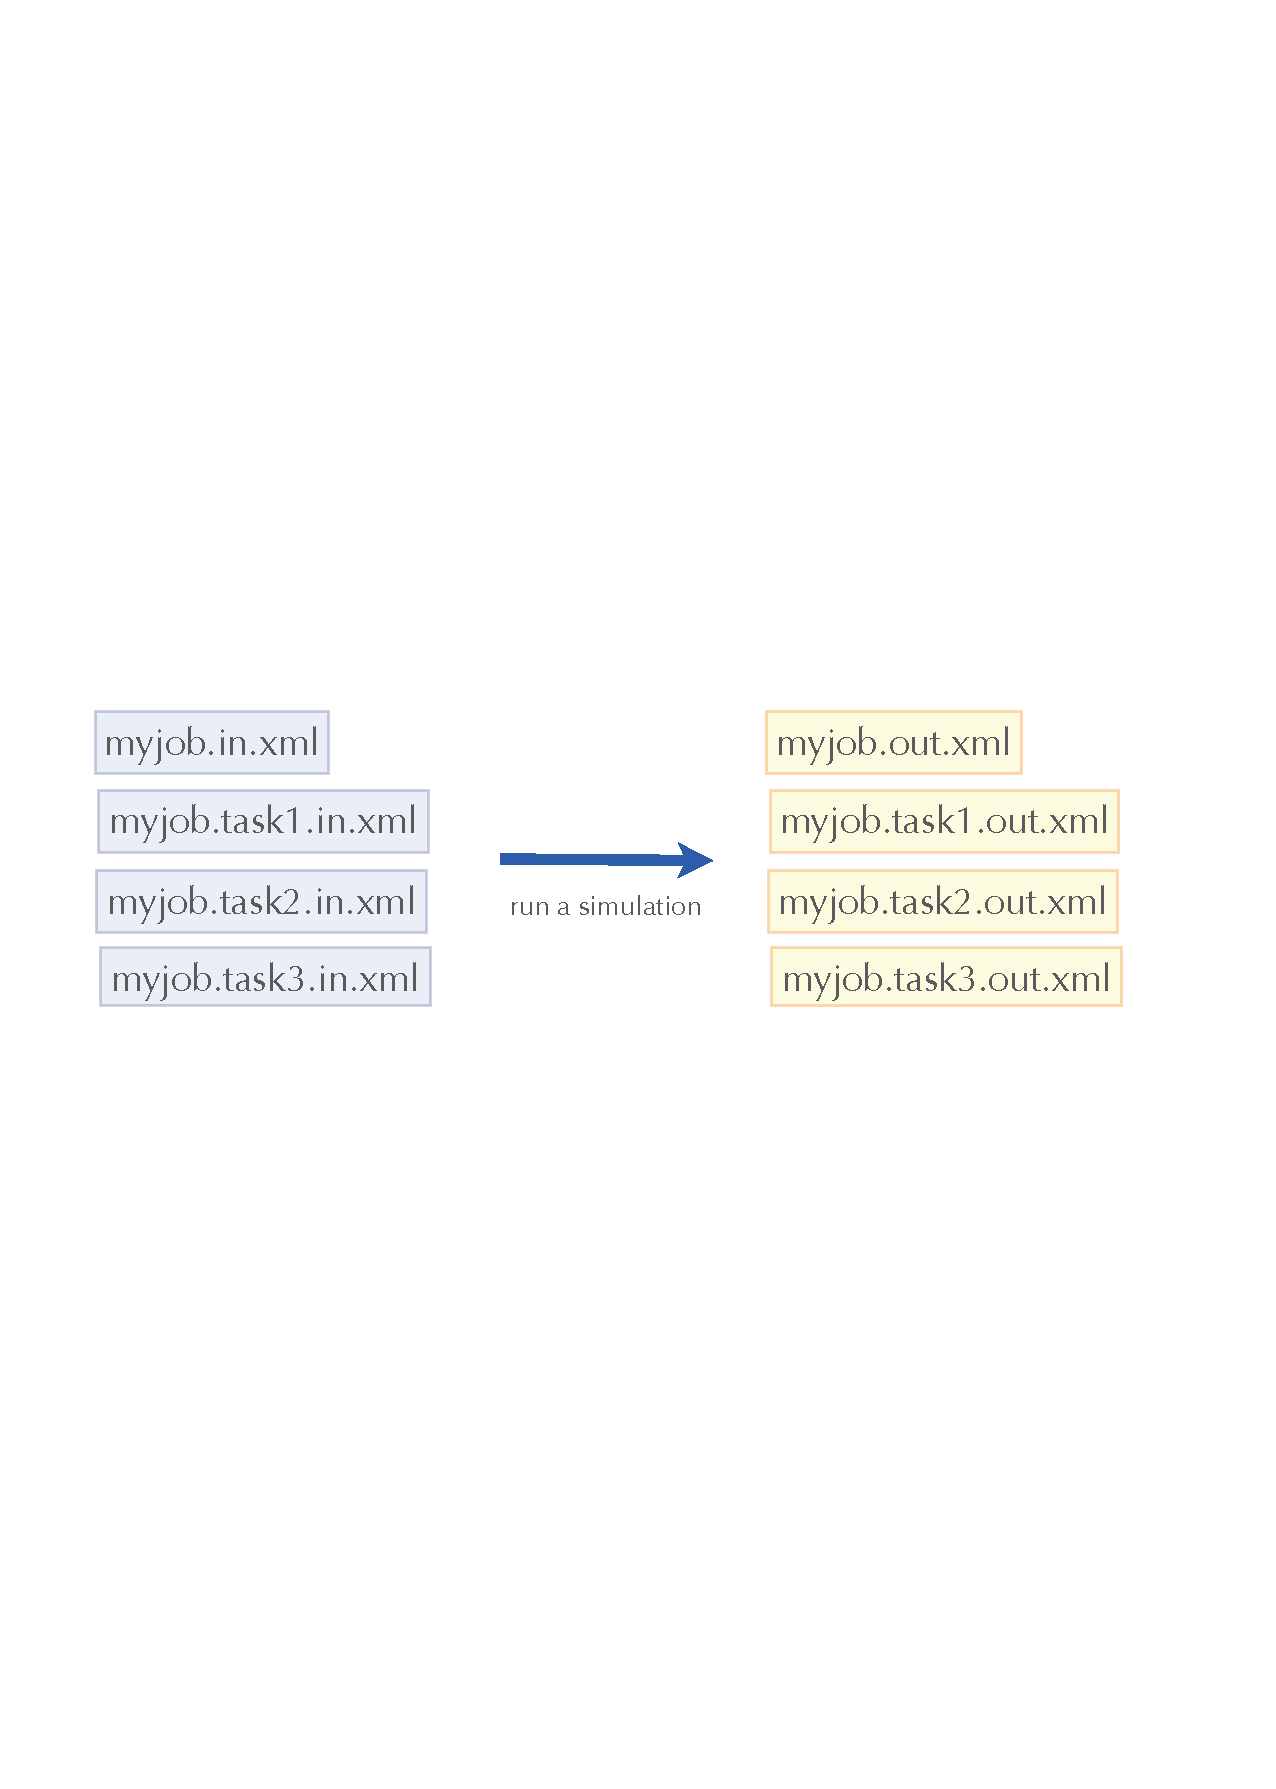
\includegraphics[width=.55\textwidth]{simulation1.pdf}
  \end{center}
  \end{itemize}
\end{frame}

\begin{frame}{Job XML ファイル}
  \begin{center}
    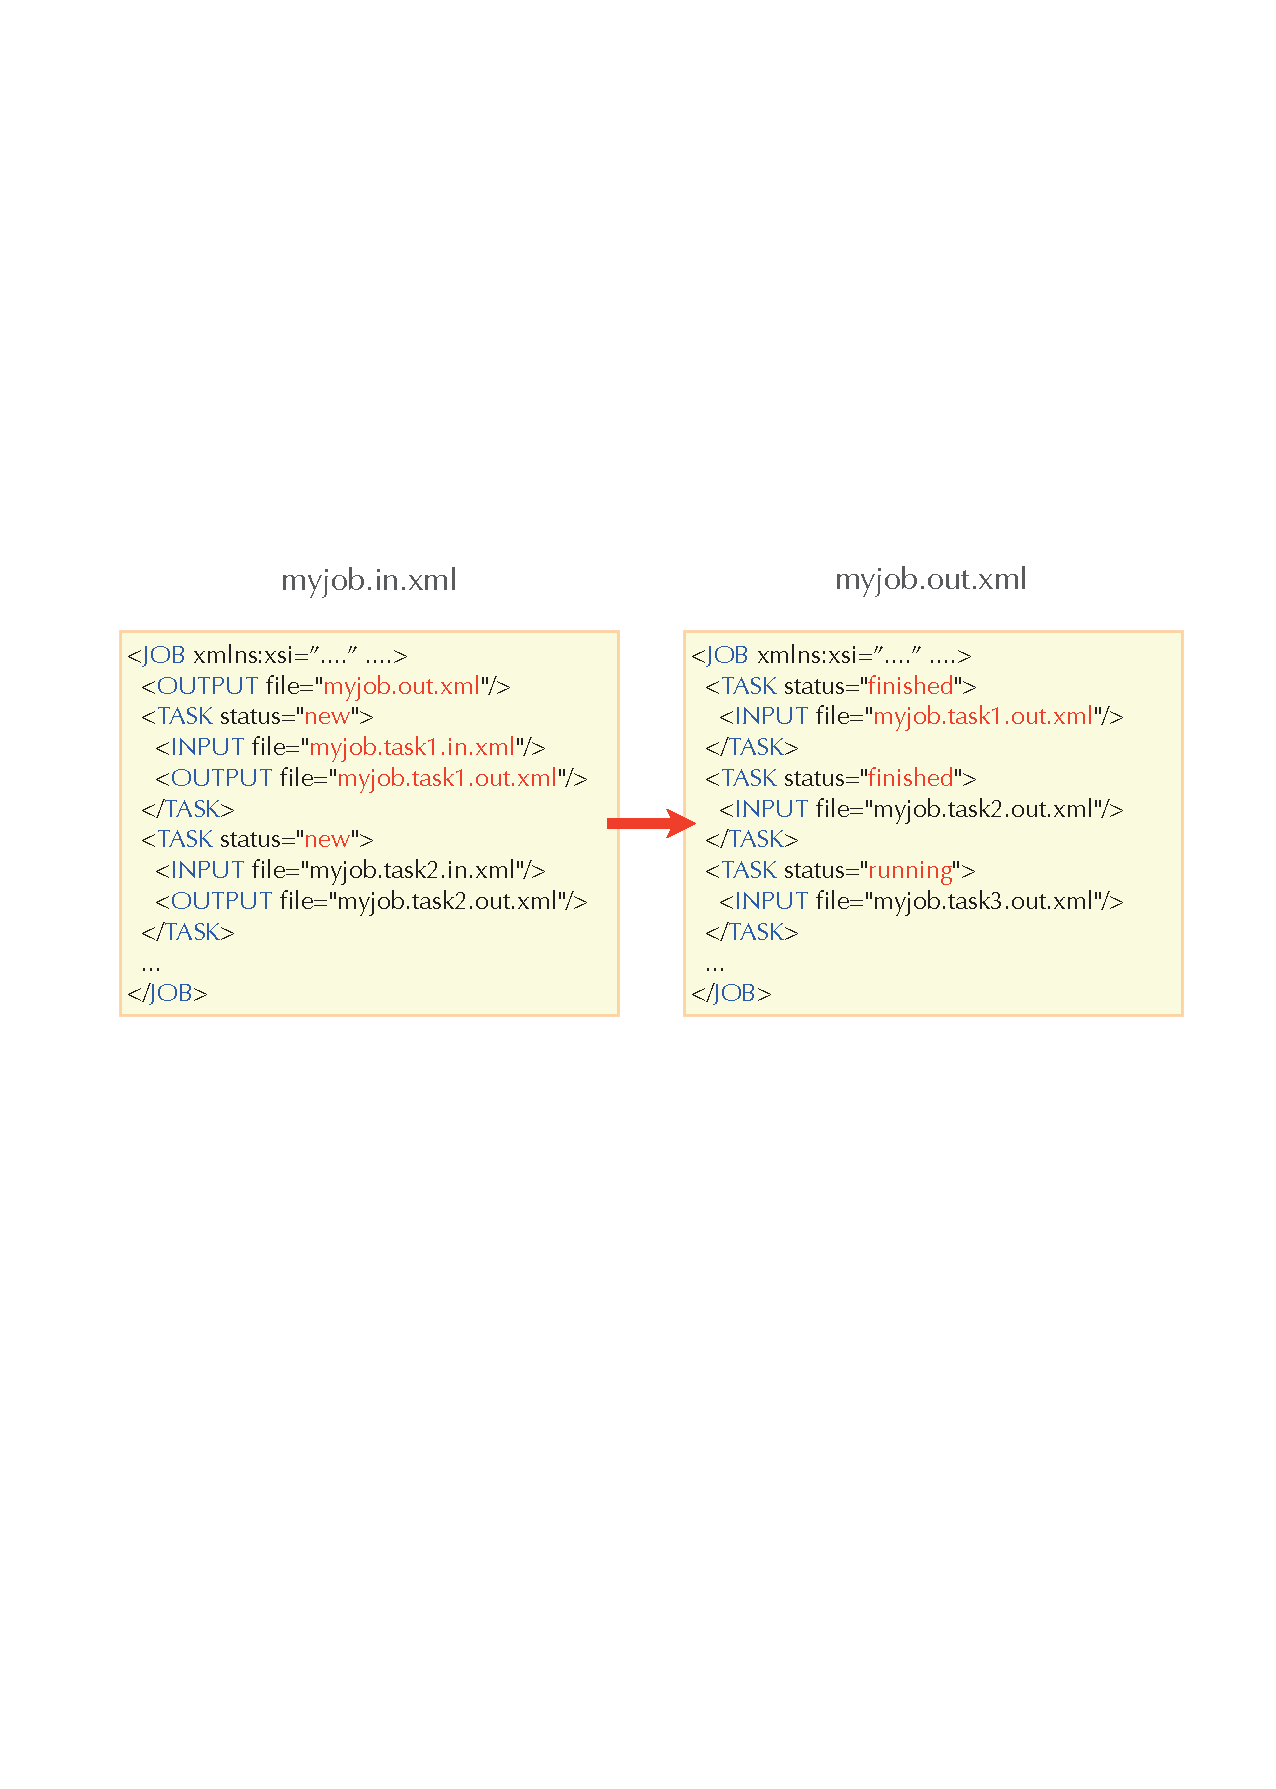
\includegraphics[height=.6\textheight]{simulation2.pdf}
  \end{center}
\end{frame}

\begin{frame}{Task XML ファイル}
  \begin{center}
    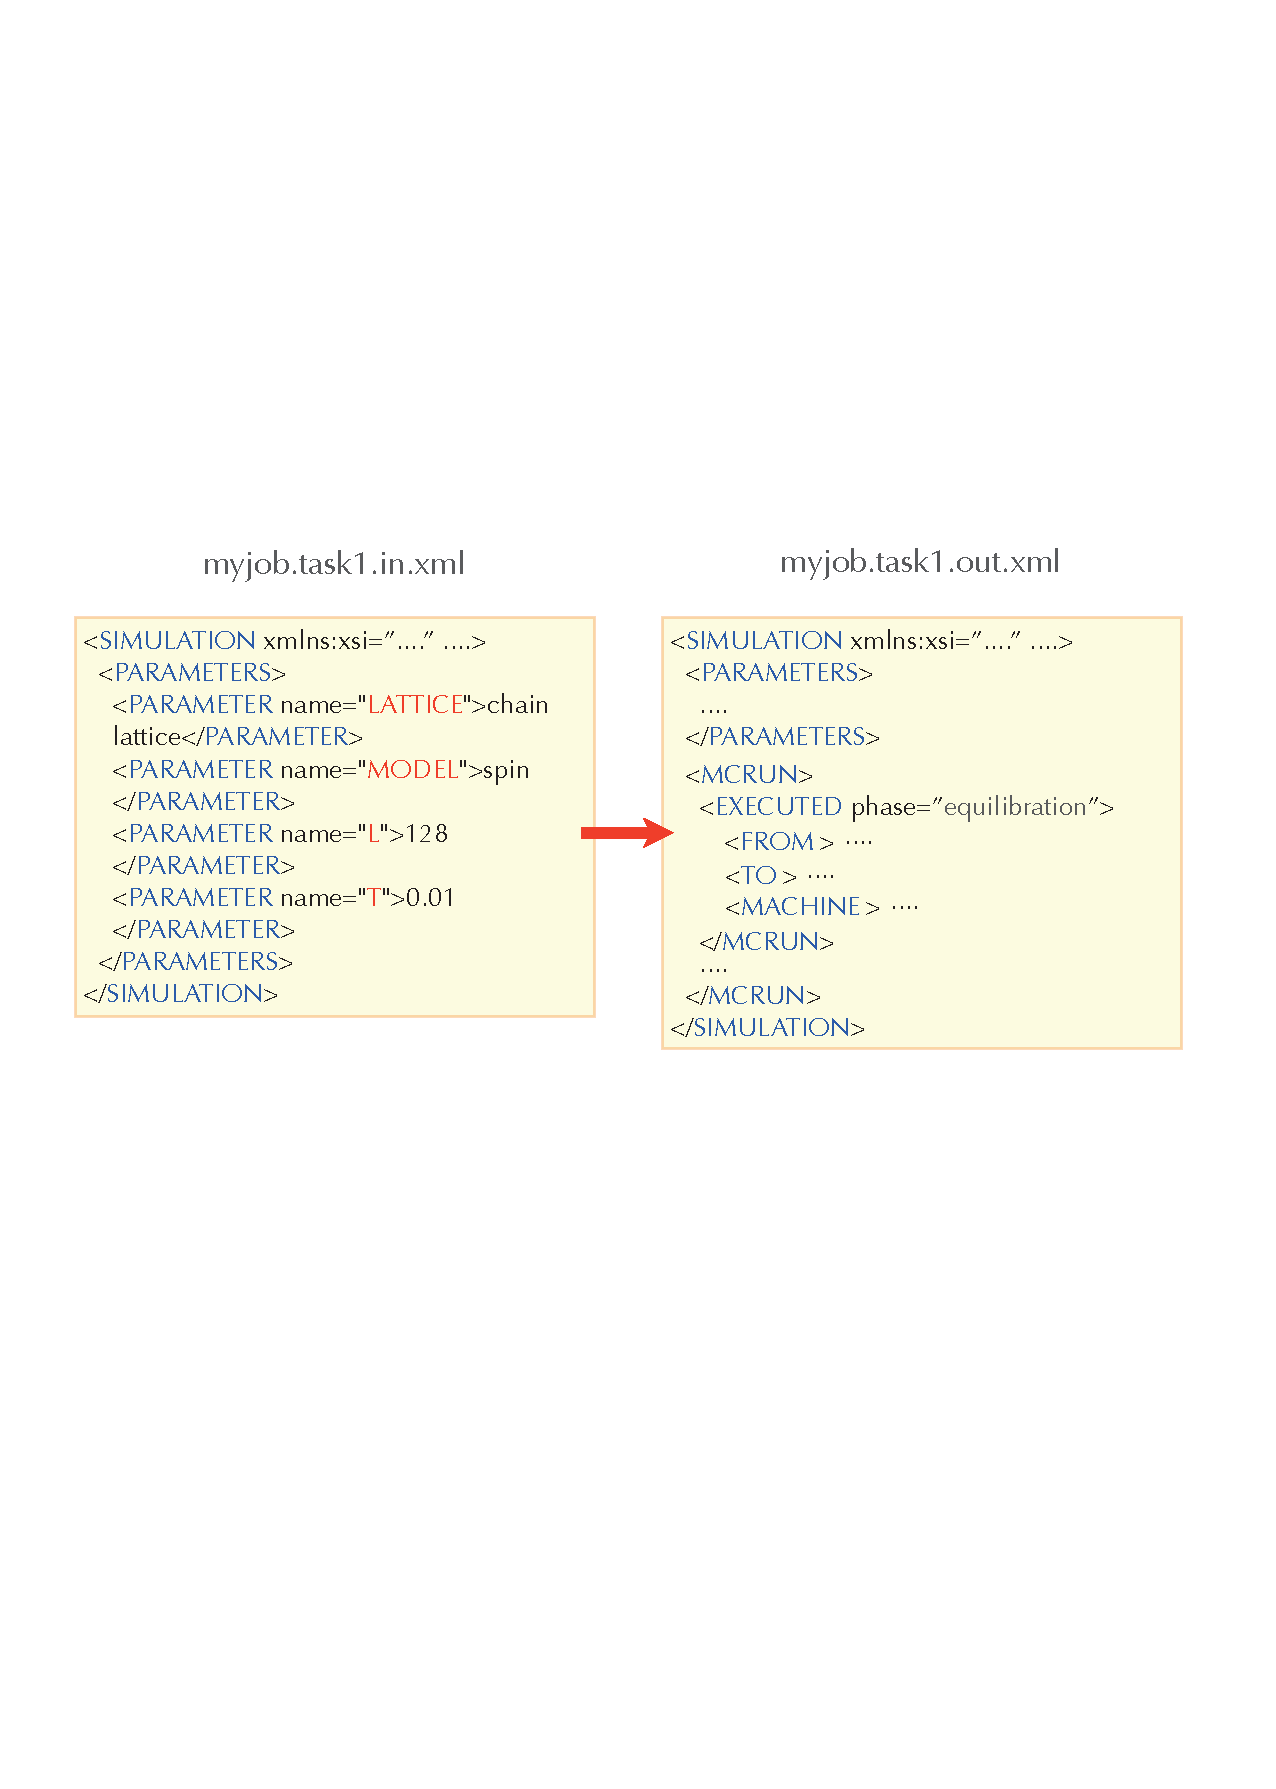
\includegraphics[height=.6\textheight]{simulation3.pdf}
  \end{center}
\end{frame}

\begin{frame}{parameter2xml ツール}
  \begin{itemize}
  \item パラメータセットを簡易形式で書いて、parameter2xmlツールでXMLに変換する
  \begin{center}
    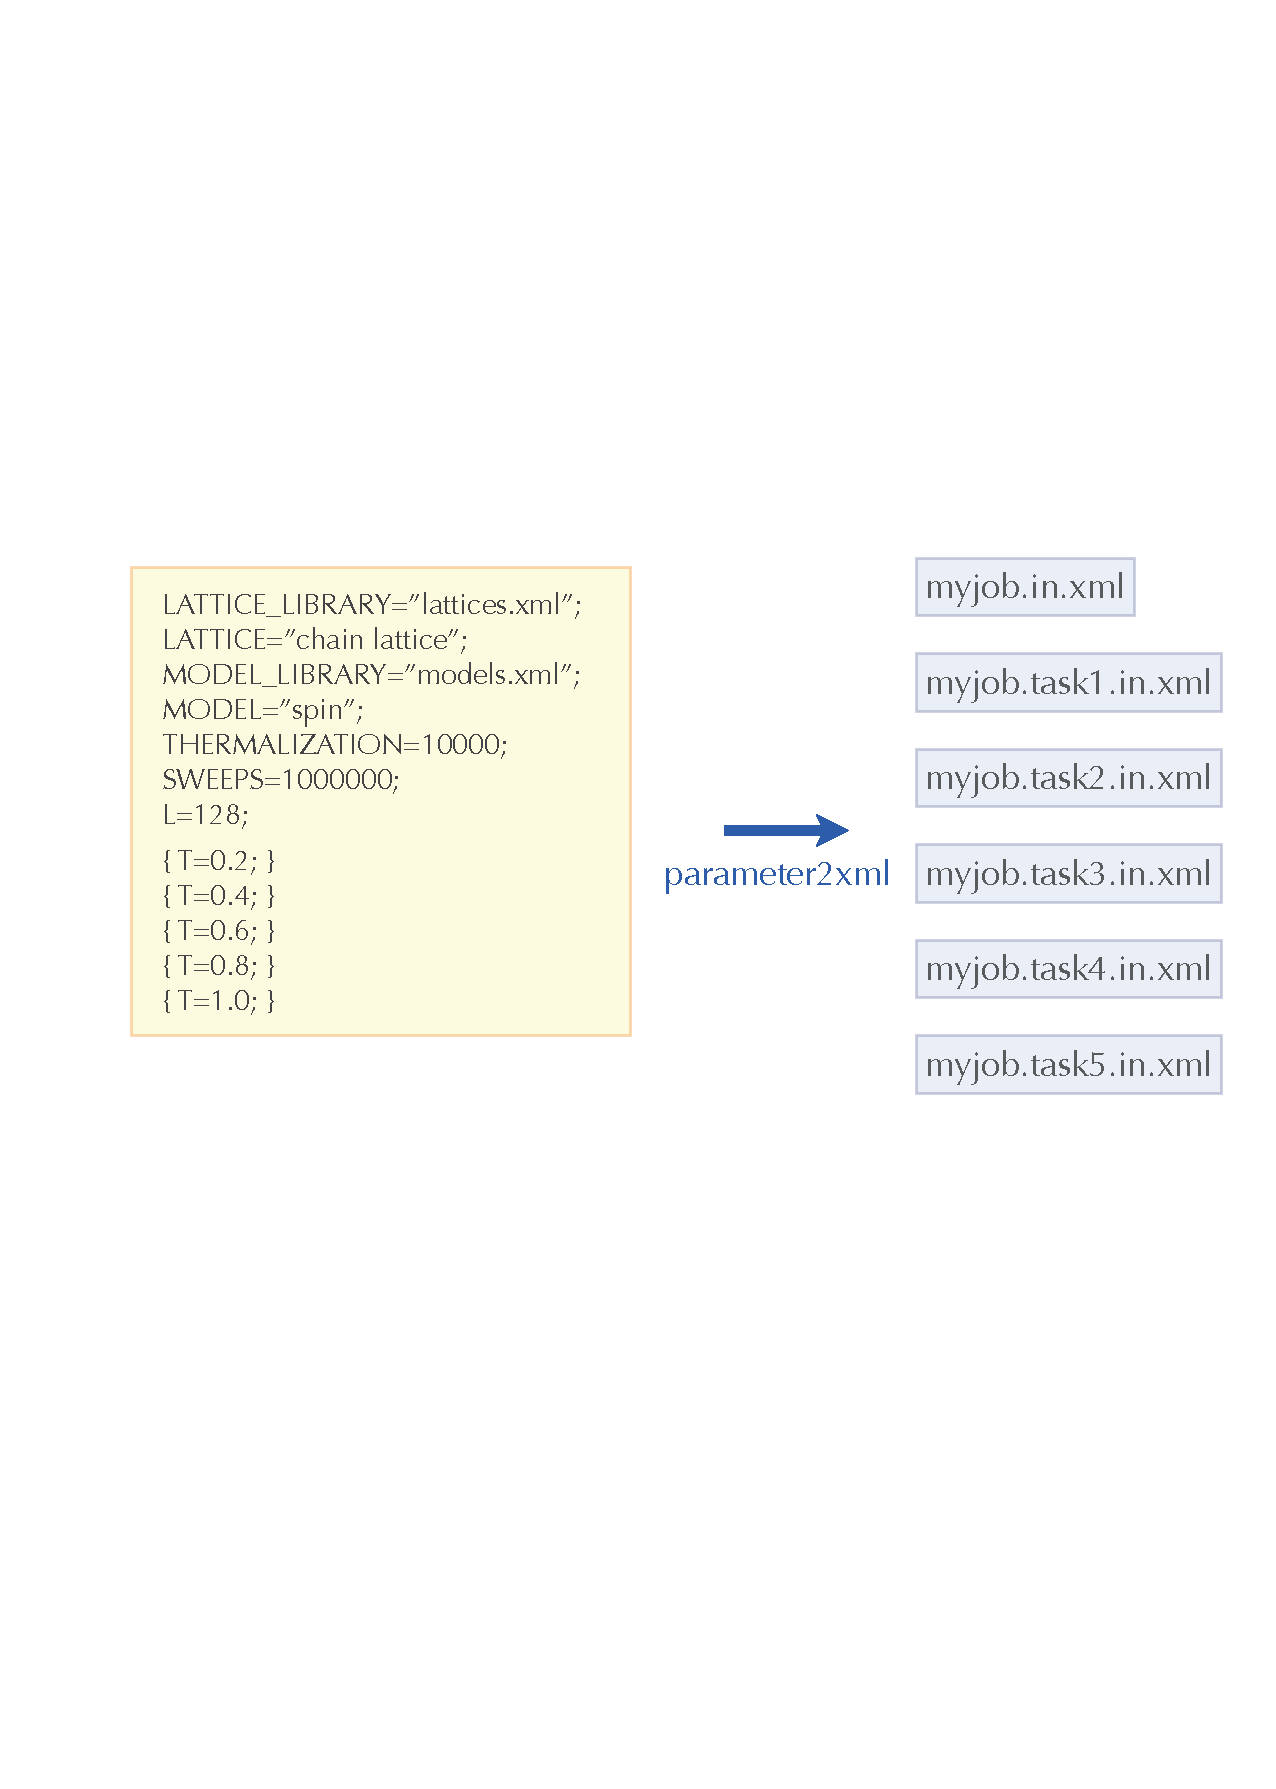
\includegraphics[height=.6\textheight]{simulation4.pdf}
  \end{center}
  \item pyalps (後述)では、pyalps.writeInputFiles() メソッドが利用できる
  \end{itemize}
\end{frame}

\begin{frame}{格子とモデルの指定}
  \begin{itemize}
  \item 格子とモデルを指定するための特別なパラメータ
  \begin{center}
    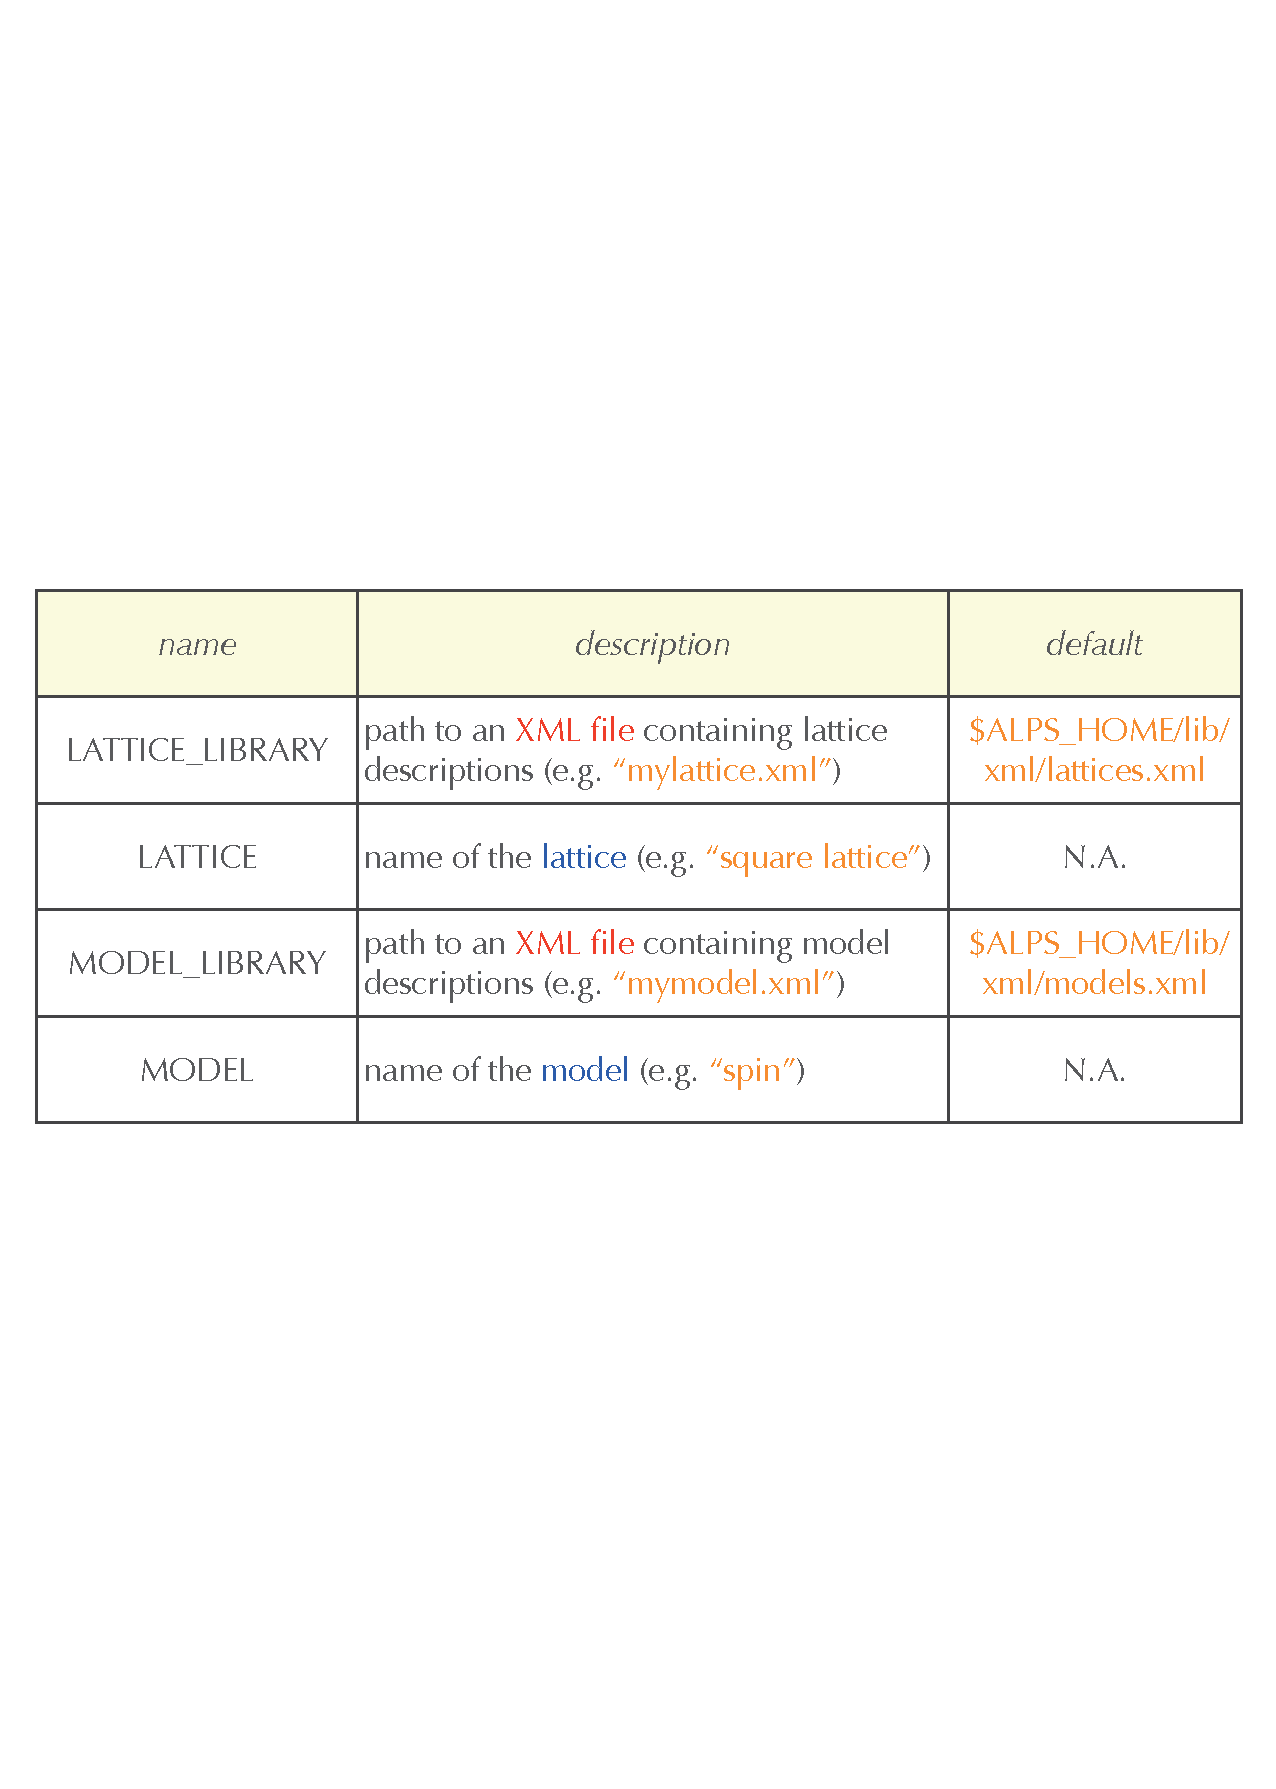
\includegraphics[height=4cm]{simulation5.pdf}
  \end{center}
  \end{itemize}
\end{frame}

\begin{frame}[t,fragile]
  \frametitle{パラメータファイルでの数式の使用}
  \begin{columns}[T]
    \begin{column}{.5\textwidth}
      \begin{itemize}
      \item パラメータの入出力のためのライブラリ
        %\begin{itemize}
        \item 改行, セミコロン, コンマで変数を区別
        \item 四則演算、初等関数(sin, cos, expなど)が使える
        \item $\pi$ (PI), 虚数単位(I)などを文字で指定
        \item C 風, C++風のコメント
        \item \{ \} で囲んだ変数は異なるセット
        \item 「循環参照」がある場合にはエラーになる
        %\end{itemize}
      \end{itemize}
    \end{column}
    \begin{column}{.5\textwidth}
    \begin{lstlisting}
LATTICE = "chain lattice";
L = 16,
SEED = 2873
// C++ style comment
SWEEPS = 4096;
THERMALIZATION = SWEEPS/8;
/* C style comment */
{ T = 2; Sq = 2*PI/3; }
{ T = 1.8; }
    \end{lstlisting}
    \end{column}
  \end{columns}
\end{frame}

\section{ALPSチュートリアル}

\begin{frame}
  \frametitle{ディレクトリ構成}
  \begin{tabular}{ll}
    /opt/nano/alps/alpsvars.sh & \\
    \hspace*{3em} ALPS環境変数(\$ALPS\_HOME等)設定スクリプト \\
    \$ALPS\_HOME/tutorials & \\
    \hspace*{3em} アプリケーションのチュートリアル用入出力ファイル \\
    \$ALPS\_HOME/tutorials/alpsize-* & \\
    \hspace*{3em} ALPS化のチュートリアル (20130501-r5861以降)
  \end{tabular}
  \begin{alertblock}{}
    alpsvars.shはALPSがインストールされたスパコン全てにあります \\
    参考: {\footnotesize \url{http://todo.issp.u-tokyo.ac.jp/ja/members/wistaria/log/alps-preinstalled}}
\end{alertblock}
\end{frame}

\begin{frame}[fragile,shrink=10]
  \frametitle{準備}
  \begin{enumerate}
  \item<1-> phiへログイン
\begin{semiverbatim}
\$ ssh -X guestXX@phi.aics.riken.jp
\end{semiverbatim}
  \item<2-> 環境変数の設定
\begin{semiverbatim}
[guestXX@phi ~]\$ echo "source /opt/nano/alps/alpsvars.sh" >> ~/.bashrc
\end{semiverbatim}
  \item<3-> phiXXへログイン
\begin{semiverbatim}
[guestXX@phi ~]\$ ssh -X phiXX
\end{semiverbatim}
  \item<4-> 本日利用するチュートリアルをコピー
\begin{semiverbatim}
[guestXX@phiXX ~]\$ cp -r \$ALPS\_HOME/tutorials/mc-02-susceptibilities .
[guestXX@phiXX ~]\$ cp -r \$ALPS\_HOME/tutorials/mc-03-magnetization .
\end{semiverbatim}
  \end{enumerate}
  \begin{alertblock}{ALPS wikiのチュートリアル}
    \url{http://alps.comp-phys.org/mediawiki/index.php/ALPS_2_Tutorials:Overview/ja}
  \end{alertblock}
\end{frame}

\begin{frame}[fragile]
  \frametitle{ALPSの実行シナリオ}
  \begin{enumerate}
  \item コマンドライン(旧来からの方法)
\begin{semiverbatim}
\$ parameter2xml \textit{param}
\$ loop \textit{param}.in.xml
\end{semiverbatim}
  \item Python (新しい方法)
    \begin{itemize}
    \item パラメータの準備からグラフ作成まで統一的に
    \item 対話的にもバッチコマンドとしても実行可能
    \item 現在、グラフの作成にはPythonを用いる
    \end{itemize}
  \item VisTrails
  \end{enumerate}
  \begin{columns}
    \begin{column}{.7\textwidth}
      \begin{center}
        \begin{alertblock}{}
          Python(ipython)での対話的実行
        \end{alertblock}
      \end{center}
    \end{column}
  \end{columns}
\end{frame}

\begin{frame}
  \frametitle{ALPSアプリケーションの一覧}
  \begin{description}
  \item[spinmc] 古典モンテカルロ法
  \item[loop] 量子モンテカルロ法(ループアルゴリズム)
  \item[dirloop\_sse] 量子モンテカルロ(向きつきループアルゴリズム)
  \item[worm] 量子モンテカルロ(ワームアルゴリズム)
  \item[sparsediag] 厳密対角化(Lanczos法)
  \item[fulldiag] 厳密対角化(全対角化法)
  \item[dmrg] 密度行列繰り込み群法
  \item[dmft] 動的平均場法
  \end{description}
\end{frame}

\begin{frame}[fragile]
  \frametitle{ALPSチュートリアル: MC-02 (1)}
  \begin{enumerate}
  \item<1-> Xの転送ができるか確認
\begin{semiverbatim}
 \$ gnome-about
\end{semiverbatim}
  \item<1-> Pythonの実行
\begin{semiverbatim}
 \$ cd mc-02-susceptibilities
 \$ ipython
\end{semiverbatim}
  \end{enumerate}
  \begin{center}
    \begin{alertblock}{}
      途中まで打ってTABで補完できます
    \end{alertblock}
  \end{center}
\end{frame}

\begin{frame}[fragile,shrink=5]
  \frametitle{ALPSチュートリアル: MC-02 (2)}
  \begin{enumerate}
  \item<2-> ALPS共通の準備
\begin{semiverbatim}
In [1]: import pyalps
\end{semiverbatim}
  \item<3-> グラフの生成(Xで表示)
\begin{semiverbatim}
In [2]: import matplotlib.pyplot as plt
In [3]: import pyalps.plot
...
In [10]: plt.show()
\end{semiverbatim}
  \item<3-> 直接PDFの生成
\begin{semiverbatim}
In [2]: import matplotlib
In [3]: matplotlib.use('PDF')
In [4]: import matplotlib.pyplot as plt
In [5]: import pyalps.plot
...
In [13]: plt.savefig('out.pdf')
\end{semiverbatim}
  \end{enumerate}
\end{frame}

\begin{frame}
  \frametitle{ALPSチュートリアル: MC-02 (3)}
  \begin{center}
    \begin{block}{}
      コマンドラインからの実演
    \end{block}
    \begin{block}{}
      Pythonからの実演
    \end{block}
  \end{center}
\end{frame}

\begin{frame}{実行結果の確認}
  \begin{itemize}
    \item 実行結果(JOB XMLファイル、TASK XMLファイル)は、webブラウザで直接開いて中身を見ることも可能
      \begin{itemize}
      \item 例(Mac OS X): open -a safari parms2a.out.xml
      \end{itemize}
  \end{itemize}
\end{frame}

\begin{frame}{シミュレーションの並列実行}
  \begin{itemize}
    \item パラメータセットに関する並列実行が可能 (embarassingly parallel)
    \item アプリケーションによって、ALPS parallelizing スケジューラか、ALPS/parapack スケジューラのいずれかが使われている (オプション -l により確認可)
    \item ALPS parallelizaing スケジューラ (spinmc等)
      \begin{itemize}
        \item OpenMPスレッド並列には対応していない。MPI並列のみ
        \item MPI実行例(4プロセス): \\ {\tt {\color{red} mpirun -np 4} \$ALPS\_HOME/bin/spinmc {\color{red} --mpi} parm2a.in.xml}
      \end{itemize}
    \item ALPS/parapack スケジューラ (loop等)
      \begin{itemize}
        \item OpenMPスレッド並列とMPI並列に対応。デフォルトで自動的にスレッド並列実行
        \item ハイブリッド(OpenMP + MPI)実行例(4プロセス16スレッド): \\ {\tt {\color{red} mpirun -np 4} \$ALPS\_HOME/bin/loop {\color{red} --mpi} {\color{red} -r 16} parm2c.in.xml}
      \end{itemize}
  \end{itemize}
\end{frame}

\section{ALPS Lattice \& Model チュートリアル}

\begin{frame}{ALPS Latticeチュートリアル}
  ALPS Lattice HowTo: {\footnotesize \url{http://alps.comp-phys.org/mediawiki/index.php/Tutorials:LatticeHOWTO/ja}} \\
  \begin{itemize}
    \item \href{http://alps.comp-phys.org/mediawiki/index.php/Tutorials:LatticeHOWTO:SimpleGraphs/ja}{辺と頂点を単位として簡単なグラフを指定する方法}
    \item \href{http://alps.comp-phys.org/mediawiki/index.php/Tutorials:LatticesAndUnitCells/ja}{格子と単一セルを指定する方法}
    \item \href{http://alps.comp-phys.org/mediawiki/index.php/Tutorials:LatticesAndGraphs/ja}{単位格子に対応するグラフを指定する方法}
    \item \href{http://alps.comp-phys.org/mediawiki/index.php/Tutorials:LatticeHOWTO:Library/ja}{格子とグラフのライブラリの生成方法}
    \item \href{http://alps.comp-phys.org/mediawiki/index.php/Tutorials:LatticeHowto:CheckLattice/ja}{格子の定義から生成されたグラフを確認する方法}
      \begin{itemize}
      \item lattice2xmlツール、あるいは(wxPythonとVTKがインストールされている環境では) lattice-preview 格子可視化ツールも利用可
      \end{itemize}
  \end{itemize}
\end{frame}

\begin{frame}{ALPS Modelチュートリアル}
  ALPS Model HowTo: {\footnotesize \url{http://alps.comp-phys.org/mediawiki/index.php/Tutorials:ModelHOWTO/ja}} \\
  \begin{itemize}
  \item \href{http://alps.comp-phys.org/mediawiki/index.php/Tutorials:ModelHOWTO/ja\#.E3.83.87.E3.83.95.E3.82.A9.E3.83.AB.E3.83.88.E3.81.AE.E3.83.A2.E3.83.87.E3.83.AB.E3.83.A9.E3.82.A4.E3.83.96.E3.83.A9.E3.83.AA.E3.83.95.E3.82.A1.E3.82.A4.E3.83.AB.E3.80.80}{デフォルトのモデルライブラリファイル}
  \item \href{http://alps.comp-phys.org/mediawiki/index.php/Tutorials:ModelHOWTO/ja\#.E3.83.A2.E3.83.87.E3.83.AB.E3.83.A9.E3.82.A4.E3.83.96.E3.83.A9.E3.83.AA.E3.83.95.E3.82.A1.E3.82.A4.E3.83.AB.E3.81.AE.E6.A7.8B.E9.80.A0}{モデルライブラリファイルの構造}
  \item \href{http://alps.comp-phys.org/mediawiki/index.php/Tutorials:ModelHOWTO/ja\#.E5.8D.98.E4.B8.80.E3.82.B5.E3.82.A4.E3.83.88.E3.81.AE.E5.9F.BA.E5.BA.95}{単一サイトの基底}
  \item \href{http://alps.comp-phys.org/mediawiki/index.php/Tutorials:ModelHOWTO/ja\#.E5.AE.8C.E5.85.A8.E6.A0.BC.E5.AD.90.E3.83.A2.E3.83.87.E3.83.AB.E3.81.AE.E5.9F.BA.E5.BA.95}{完全格子モデルの基底}
  \item \href{http://alps.comp-phys.org/mediawiki/index.php/Tutorials:ModelHOWTO/ja\#.E9.87.8F.E5.AD.90.E6.BC.94.E7.AE.97.E5.AD.90}{量子演算子}
  \item \href{http://alps.comp-phys.org/mediawiki/index.php/Tutorials:ModelHOWTO/ja\#.E3.83.8F.E3.83.9F.E3.83.AB.E3.83.88.E3.83.8B.E3.82.A2.E3.83.B3.E3.81.AE.E5.8F.96.E6.89.B1.E3.81.84}{ハミルトニアンの取扱い}
  \end{itemize}
\end{frame}

\end{document}

%%% Local Variables: 
%%% mode: japanese-latex
%%% TeX-master: nil
%%% coding: utf-8
%%% End: 
